% I seguenti commenti speciali impostano:
% 1. utf8 come codifica di input,
% 2. PDFLaTeX come motore di composizione;
% 3. Articolo.tex come documento principale;
% 4. il controllo ortografico italiano per l'editor.

% !TEX encoding = UTF-8
% !TEX TS-program = pdflatex
% !TEX root = Articolo.tex
% !TEX spellcheck = it-IT

\documentclass[10pt,%                       % corpo del font principale
               a4paper,%                    % carta A4
%              oneside,%                    % solo fronte
               twoside,%                    % fronte-retro
               ]{article}                   % classe report di KOMA-Script;
               
\usepackage[T1]{fontenc}                    % codifica dei font:
                                            % NOTA BENE! richiede una distribuzione *completa* di LaTeX,
                                            % per esempio TeXLive o MiKTeX *complete*

\usepackage[utf8]{inputenc}                 % codifica di input; anche [latin1] va bene
                                            % NOTA BENE! va accordata con le preferenze dell'editor

\usepackage[english,italian]{babel}         % per scrivere in italiano e in inglese;
                                            % l'ultima lingua (l'italiano) risulta predefinita

\usepackage[binding=5mm]{layaureo}          % margini ottimizzati per l'A4; rilegatura di 5 mm

\usepackage{indentfirst}                    % rientra il primo capoverso di ogni sezione

\usepackage{booktabs}                       % tabelle

\usepackage{tabularx}                       % tabelle di larghezza prefissata

\usepackage{graphicx}                       % immagini

\usepackage{subfig}                         % sottofigure, sottotabelle

\usepackage{caption}                        % didascalie

\usepackage{listings}                       % codici

\usepackage[font=small]{quoting}            % citazioni

\usepackage{amsmath,amssymb,amsthm}         % matematica

\usepackage[italian]{varioref}              % riferimenti completi della pagina

\usepackage{mparhack,fixltx2e,relsize}      % finezze tipografiche

\usepackage[style=philosophy-modern,hyperref,backref,square,natbib]{biblatex}
                                            % eccellente pacchetto per la bibliografia;
                                            % produce uno stile di citazione autore-anno; 
                                            % lo stile "numeric-comp" produce riferimenti numerici
                                          
\bibliography{Bibliografia}                 % database di biblatex 
                                          
\usepackage[dvipsnames]{xcolor}             % colori

\usepackage{lipsum}                         % testo fittizio

\usepackage{eurosym}                        % simbolo dell'euro

\usepackage{hyperref}                       % collegamenti ipertestuali

\usepackage{bookmark}                       % segnalibri

\usepackage{minted}

%*********************************************************************************
% impostazioni-articolo.tex
% file che contiene le impostazioni dell'articolo
%*********************************************************************************


%*********************************************************************************
% Comandi personali
%*******************************************************
\newcommand{\myName}{Daniele Biasini \\ Alexandru Obada}                           
\newcommand{\myTitle}{\textbf{Progetto di un array lineare di patch rettangolari per base station WiMax}}
\date{}                                                           

\title{\myTitle}
\author{\myName}

\newcommand{\myDegree}{Progetto di fine corso}                       % tipo di tesi
\newcommand{\myUni}{Universit\`a degli Studi di Roma Tor Vergata} % universit\`a
\newcommand{\myFaculty}{Facolt\`a di Ingegneria delle Tecnologie di Internet}    % facolt\`a
\newcommand{\myDepartment}{Tecnologie Elettromagnetiche per Sistemi Wireless}         % dipartimento
\newcommand{\myProf}{Prof. Gaetano Marrocco}      % relatore
%\newcommand{\myOtherProf}{Dott.~Immanuel Kant}              % eventuale correlatore
\newcommand{\myLocation}{Roma}                         % dove
\newcommand{\myTime}{Gennaio 2013}                          % quando
\newcommand{\cheby}{Čebyšëv}


%*********************************************************************************
% Impostazioni di amsmath, amssymb, amsthm
%*********************************************************************************

% comandi per gli insiemi numerici (serve il pacchetto amssymb)
\newcommand{\numberset}{\mathbb} 
\newcommand{\N}{\numberset{N}} 
\newcommand{\R}{\numberset{R}} 

% un ambiente per i sistemi
\newenvironment{sistema}%
  {\left\lbrace\begin{array}{@{}l@{}}}%
  {\end{array}\right.}

% definizioni (serve il pacchetto amsthm)
\theoremstyle{definition} 
\newtheorem{definizione}{Definizione}

% teoremi, leggi e decreti (serve il pacchetto amsthm)
\theoremstyle{plain} 
\newtheorem{teorema}{Teorema}
\newtheorem{legge}{Legge}
\newtheorem{decreto}[legge]{Decreto}
\newtheorem{murphy}{Murphy}[section]



%*********************************************************************************
% Impostazioni di biblatex
%*********************************************************************************
\defbibheading{bibliography}{%
\phantomsection 
\addcontentsline{toc}{section}{\refname}
\section*{\bibname\markboth{\MakeUppercase{\refname}}{\MakeUppercase{\refname}}}}



%*********************************************************************************
% Impostazioni di listings
%*********************************************************************************
\lstset{language=[LaTeX]Tex,%C++,
    keywordstyle=\color{RoyalBlue},%\bfseries,
    basicstyle=\small\ttfamily,
    %identifierstyle=\color{NavyBlue},
    commentstyle=\color{Green}\ttfamily,
    stringstyle=\rmfamily,
    numbers=none,%left,%
    numberstyle=\scriptsize,%\tiny
    stepnumber=5,
    numbersep=8pt,
    showstringspaces=false,
    breaklines=true,
    frameround=ftff,
    frame=single
} 



%*********************************************************************************
% Impostazioni di hyperref
%*********************************************************************************
\hypersetup{%
    hyperfootnotes=false,pdfpagelabels,
    %draft,	% = elimina tutti i link (utile per stampe in bianco e nero)
    colorlinks=true, linktocpage=true, pdfstartpage=1, pdfstartview=FitV,%
    % decommenta la riga seguente per avere link in nero (per esempio per la stampa in bianco e nero)
    %colorlinks=false, linktocpage=false, pdfborder={0 0 0}, pdfstartpage=1, pdfstartview=FitV,% 
    breaklinks=true, pdfpagemode=UseNone, pageanchor=true, pdfpagemode=UseOutlines,%
    plainpages=false, bookmarksnumbered, bookmarksopen=true, bookmarksopenlevel=1,%
    hypertexnames=true, pdfhighlight=/O,%nesting=true,%frenchlinks,%
    urlcolor=webbrown, linkcolor=RoyalBlue, citecolor=webgreen, %pagecolor=RoyalBlue,%
    %urlcolor=Black, linkcolor=Black, citecolor=Black, %pagecolor=Black,%
    pdftitle={\myTitle},%
    pdfauthor={\textcopyright\ \myName},%
    pdfsubject={},%
    pdfkeywords={},%
    pdfcreator={pdfLaTeX},%
    pdfproducer={LaTeX with hyperref and ClassicThesis}%
}



%*********************************************************************************
% Impostazioni di graphicx
%*********************************************************************************
\graphicspath{{Immagini/}} % cartella dove sono riposte le immagini



%*********************************************************************************
% Impostazioni di xcolor
%*********************************************************************************
\definecolor{webgreen}{rgb}{0,.5,0}
\definecolor{webbrown}{rgb}{.6,0,0}



%*********************************************************************************
% Impostazioni di caption
%*********************************************************************************
\captionsetup{tableposition=top,figureposition=bottom,font=small,format=hang,labelfont=bf}



%*********************************************************************************
% Altro
%*********************************************************************************

% [...] ;-)
\newcommand{\omissis}{[\dots\negthinspace]}

% eccezioni all'algoritmo di sillabazione
\hyphenation{Fortran ma-cro-istru-zio-ne nitro-idrossil-amminico}               % file con le impostazioni personali


\begin{document}
\pagestyle{headings} 
%******************************************************************
% Materiale iniziale
%******************************************************************
% !TEX encoding = UTF-8
% !TEX TS-program = pdflatex
% !TEX root = ../Articolo.tex
% !TEX spellcheck = it-IT

%*******************************************************
% Frontespizio
%*******************************************************
%\maketitle
%\newpage

\begin{titlepage}
\pdfbookmark{Frontespizio}{Frontespizio}
%\changetext{}{}{}{((\paperwidth - \textwidth) / 2) - \oddsidemargin - \hoffset - 1in}{}
\null\vfill
\begin{center}
\large
%\sffamily
\bigskip

{\LARGE\myName} \\

\bigskip

{\Huge\myTitle \\
}

\bigskip
    
\vspace{9cm}

\begin{tabular}{cc}
\parbox{0.3\textwidth}{
\includegraphics[width=3cm]{Immagini/logo}}
&
\parbox{0.7\textwidth}{{\Large\myDegree} \\ 

					{\normalsize
					 \myProf \\
%					Co-relatore: \myOtherProf \\
%					
					\myUni \\
					\myFaculty \\
					\myDepartment \\
					\myTime}}
			\end{tabular}
\end{center}
\vfill
\end{titlepage}
% !TEX encoding = UTF-8
% !TEX TS-program = pdflatex
% !TEX root = ../Articolo.tex
% !TEX spellcheck = it-IT

%*******************************************************
% Indici
%*******************************************************
\pdfbookmark{\contentsname}{tableofcontents}
\setcounter{tocdepth}{2}
\tableofcontents
\markboth{\contentsname}{\contentsname} 

%*******************************************************
% Elenco delle figure
%*******************************************************    
\phantomsection
\pdfbookmark{\listfigurename}{lof}
\listoffigures

%*******************************************************
% Elenco delle tabelle
%*******************************************************
\phantomsection
\pdfbookmark{\listtablename}{lot}
\listoftables
\newpage
% !TEX encoding = UTF-8
% !TEX TS-program = pdflatex
% !TEX root = ../Articolo.tex
% !TEX spellcheck = it-IT

%*******************************************************
% Sommario+Abstract
%*******************************************************
\markright{}
\section*{Sommario}
In questo lavoro è stato progettato un array di antenne a patch secondo alcune specifiche assegnate dal docente. Utilizzando queste specifiche si ottiene un'antenna compatibile con la tecnologia \emph{WiMAX}. \\
Di seguito sono elencate le specifiche di progetto:
\begin{itemize}
\item $f_{0} = 5.8 GHz$
\item $B > 2\% $
\item $G_{max} = 16 dB $
\item $R = -20 dB $
\item $BW_{-3dB} \approx 10^\circ $
\end{itemize}
\newpage
%******************************************************************
% Materiale principale
%******************************************************************
\section{Modellazione del singolo patch}

\subsection{Dimensionamento del patch con il modello di \emph{Carver}}
Il primo passo verso la progettazione dell'antenna è il dimensionamento del singolo patch, per svolgere questi calcoli, ed anche i successivi, sono stati sviluppati alcuni script in \emph{Python}, ciò ha portato alcuni vantaggi come la possibilità di automatizzare le operazioni e di avere valori teorici molto precisi.
Il primo passo da compiere è la scelta del dielettrico, è stato scelto un \emph{Duroid 5880} (Fig. \ref{img:duroid}), con costante dielettrica $\epsilon_r = 2.2$ e angolo di perdita  $tan \theta = 0.0009$.
\begin{figure}
\centering
\caption{Duroid 5880.}
\label{img:duroid}
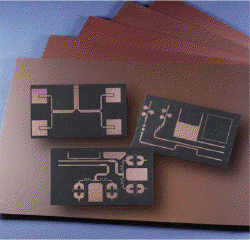
\includegraphics[scale=0.3]{Immagini/duroid}
\end{figure}

Il passo successivo è il calcolo dell'altezza massima del dielettrico che garantisce la
trascurabilità dei modi d'onda superficiali presenti nel patch a causa della discontinuità dielettrica. L'altezza scelta per il substrato dielettrico deve essere inferiore od uguale a questo valore.
\begin{align}
\label{eq:hmax}
h_{max} = \frac{0.3 c}{2 \pi f_{0} \sqrt{\epsilon_{r}}} = 1.66503477015 mm
\end{align}

Si calcola quindi la larghezza del patch:
\begin{align}
\label{eq:w}
W = \frac{c}{2f_0}\sqrt{\frac{2}{\epsilon_r+1}} = 20.4457607338 mm 
\end{align} 

\begin{minted}[linenos=true,frame=leftline,xleftmargin=0.5cm,fontsize=\footnotesize]{python}
# Velocita' della luce [m/s]
c = 3*10**8
# Imedenza del cavo coassiale [Ohm]
r = 50
# Costante dielettrica del Duroid 5880
epsilon_r = 2.2
# Frequenza di risonanza [Hz]
f = 5.8*10**9
# Altezza massima del substrato [mm]
h_max = (0.3*c)/(2*cmath.pi*f*cmath.sqrt(epsilon_r)).real
# Larghezza del patch [mm]
w = (c/(2*f)*cmath.sqrt(2/(epsilon_r+1))).real
\end{minted}

A questo punto è possibile utilizzare $h_{max}$(\ref{eq:hmax}) e $W$(\ref{eq:w}) per ottenere le altre dimensioni del patch. \\
Lo script sviluppato contiene i parametri del \emph{Duroid 5880}, e, inserito un valore per lo spessore $h$ del substrato inferiore a quello calcolato (\ref{eq:hmax}), calcola automaticamente la lunghezza del patch e del punto di alimentazione. \\
\begin{minted}[linenos=true,frame=leftline,xleftmargin=0.5cm,fontsize=\footnotesize]{python}
h = get_h(h_max)
\end{minted}

\begin{minted}[linenos=true,frame=leftline,xleftmargin=0.5cm,fontsize=\footnotesize]{python}
def get_h(h_m):
    while(True):
        h = float(input("introdurre lo spessore del substrato (minore di" + str(h_m*1000)+" mm) \n"))
        if h > 0 and h < h_m*1000:
            return h/1000
\end{minted}
La lunghezza del patch può essere ottenuta mediante la formula successiva:
\begin{align}
L = \frac{c}{2f_0\sqrt{\epsilon_r}} - 2 \Delta L = 16.8984183063 mm 
\end{align}
dove: 
\begin{itemize}
\item Estensione del campo di Fringe :
$\begin{aligned}
\Delta L = 0.412 h \frac{(\epsilon_{eff}+0.3)(\frac{W}{h}+0.264)}{(\epsilon_{eff}-0.258)(\frac{W}{h}+0.8)} 
\end{aligned}$
\item Costante dielettrica efficace:
$\begin{aligned}
\epsilon_{eff} = \frac{\epsilon_r+1}{2} + \frac{\epsilon_r-1}{2} (1 + \frac{h}{W})^{-1}
\end{aligned}$
\item Lunghezza d'onda:
$\begin{aligned}
\lambda = \frac{\lambda_0}{\sqrt{\epsilon_{eff}}}
\end{aligned}$
\end{itemize}

\begin{minted}[linenos=true,frame=leftline,xleftmargin=0.5cm,fontsize=\footnotesize]{python}
lunghezza = getLength(w,h,c,f,epsilon_r)
\end{minted}
\begin{minted}[linenos=true,frame=leftline,xleftmargin=0.5cm,fontsize=\footnotesize]{python}
def getLength(w, h , c , f , epsilon_r):
    # Costante dielettrica efficace
    epsilon_eff = ((epsilon_r+1) + (epsilon_r-1)*(1+12*h/w)**(-0.5))/2
    delta_l = h * 0.412 * ( epsilon_eff + 0.3 )*( w/h + 0.264 )/((epsilon_eff - 0.258 )*( w/h + 0.8 ))
    l = c/( 2 * f * cmath.sqrt(epsilon_eff) ) - 2 * delta_l
    return l.real
\end{minted}

Infine si calcola il punto di alimentazione:
\begin{align}
l_a = \frac{1}{\beta} arccos\biggr(\sqrt{\frac{R_{in}}{R}}\biggr) = 5.32528400943 mm
\end{align}

dove: 
\begin{itemize}
\item Costante di fase:
$\begin{aligned}
\beta = \frac{2 \pi \sqrt{\epsilon_r}}{\lambda_0} 
\end{aligned}$
\item Impedenza d'ingresso desiderata:
$\begin{aligned}
R_{in} = 50 \Omega
\end{aligned}$
\item Resistenza di radiazione:
$\begin{aligned}
R_r = \frac{1}{2G_s} = \frac{60 \lambda_0}{W} \biggr[ 1-\frac{1}{24} \biggr( \frac{2 \pi h}{\lambda_0} \biggr) ^2 \biggr] ^{-1}
\end{aligned}$
\end{itemize}
\begin{minted}[linenos=true,frame=leftline,xleftmargin=0.5cm,fontsize=\footnotesize]{python}
l_alimentazione = getFeedPoint(f , h , w , r , c , epsilon_r )
\end{minted}

\begin{minted}[linenos=true,frame=leftline,xleftmargin=0.5cm,fontsize=\footnotesize]{python}
def getFeedPoint(f , h , w , r , c , epsilon_r):
    lambda_0 = c/f
    r_r = 60*lambda_0/w * (1 - 1/24*(2*cmath.pi*h/lambda_0)**2)**(-1)
    l = lambda_0 / (2*cmath.pi * cmath.sqrt(epsilon_r))*cmath.acos(cmath.sqrt(r/r_r))
    return l.real
\end{minted}

L'output dello script mostrato in frammenti nel paragrafo è un file di testo con tutte le informazioni utili per poter realizzare il singolo patch con \emph{FEKO}.

\begin{minted}[linenos=true,frame=leftline,xleftmargin=0.5cm,fontsize=\footnotesize]{python}
h = 1.0 mm 
la = 5.32528400943 mm 
W = 20.4457607338 mm 
h_max = 1.66503477015 mm 
L = 16.8984183063 mm 
\end{minted}

\subsection{Creazione del modello del patch con FEKO}
\subsubsection*{Modello teorico}
Una volta ottenute le dimensioni del patch è possibile realizzarne un modello tridimensionale attraverso l'uso del CAD elettrmagnetico \emph{FEKO}, nella figura \ref{img:patch} è mostrato il patch realizzato.
\begin{figure}
\centering
\caption{Patch realizzato in FEKO con le relative dimensioni.}
\label{img:patch}
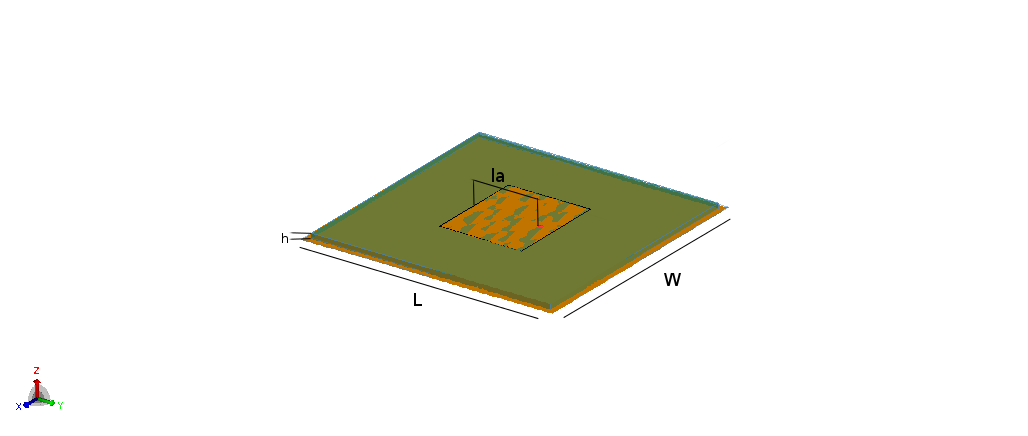
\includegraphics[scale=0.5]{Immagini/patch_original_dim}
\end{figure}

Con l'utilizzo di \emph{POSTFEKO} è possibile rielaborare i dati precedenti per ottenere informazioni riguardo al patch, si è scelto di rappresentare il coefficiente di riflessione e l'impedenza di ingresso. \\
Nella figura \ref{img:reflori} è mostrata l'attenuazione del coefficiente di riflessione, come evidenziato nella figura, si può notare che c'è un minimo in $5.81167 GHz$ a $-8.83847 dB$, inoltre alla frequenza di risonanza $f_0 = 5.8 GHz$ l'attenuazione è di $-8.82411 dB$. \\
I valori conseguiti non rispettano le specifiche di progetto, inoltre non è neanche possibile calcolare la banda percentuale a $-15 dB$.
\begin{figure}
\centering
\caption{Coefficiente di riflessione relativo alla configurazione teorica del patch.}
\label{img:reflori}
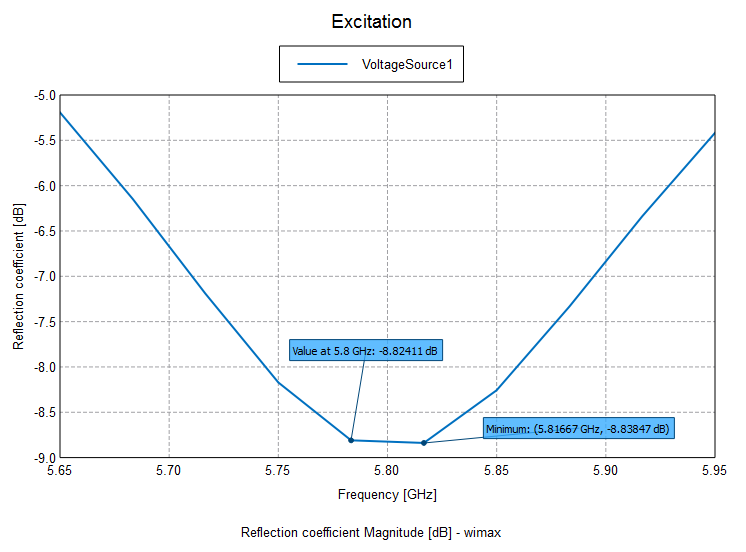
\includegraphics[scale=0.5]{Immagini/reflection_coefficient_original}
\end{figure}

La figura \ref{img:impori} mostra i valori dell'impedenza d'ingresso alla frequenza di risonanza: la parte reale dell'impedenza è di $\Re{[Z]} = 51.1 \Omega $, la parte immaginaria è di  $\Im{[Z]} = -38.3 \Omega$. La parte reale andrebbe bene ma la parte immaginaria ad un valore così alto porterebbe a ingenti perdite di potenza.

\begin{figure}
\centering
\caption{Parte reale e parte immaginaria dell'impedenza relative alla configurazione teorica del patch.}
\label{img:impori}
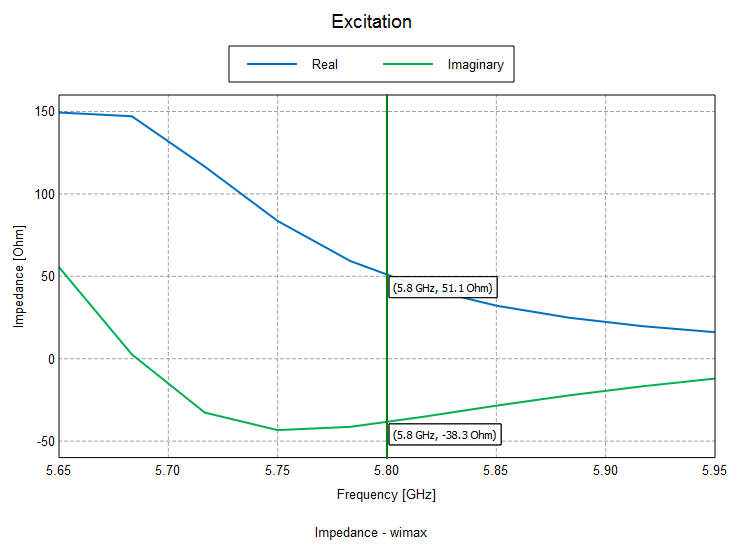
\includegraphics[scale=0.5]{Immagini/impedance_original}
\end{figure}

\subsubsection*{Ottimizzazione del modello teorico}
I risultati ottenuti con i modelli teorici mostrano come non solo non siano soddisfatte le specifiche di progetto ma anche come, volendo utilizzare tale modello, si ottengano bassissime prestazioni. \\
Per ottimizzare il modello teorico è necessario variare i valori dati in input a \emph{POSTFEKO}: le dimensioni del patch. Riuscendo quindi a cambiare opportunamente $W$, $L$, $la$ e $h$ è possibile adempiere alle specifiche di progetto, le quali riferendosi al momento al singolo patch, si traducono nell'ottenere un'\emph{attenuazione del coefficiente di riflessione inferiore a 15 dB}, portare la \emph{parte reale dell'impedenza di ingresso ad un valore prossimo allo zero} e nell'avere \emph{una banda percentuale superiore al 2\%}. \\
La realizzazione di ognuna delle specifiche non è indipendente l'una dall'altra, spesso, infatti, il soddisfacimento di una specifica porta al peggioramento di un'altra. Quindi anche la variazione di alcune dimensioni del patch porta a variazioni, anche molto diverse, dei tre obiettivi da raggiungere. \\
Dopo numerose prove, sono stati scelte le seguenti dimensioni (tabella \ref{tab:confronto}) che porteranno ai risultati mostrati nelle figure \ref{img:reflopt}, \ref{img:impopt}, \ref{img:polar}.

\begin{table}[h]\footnotesize
\caption{Confronto tra i valori teorici e quelli ottimizzati.}
\label{tab:confronto}
\begin{tabularx}{\textwidth}{XXXXXX}
\toprule
Valori & $h(m)$ & $L(m)$ & $l_a(m)$ & $W(m)$ \\
\midrule
Teorici & 1 & 16.8984183063 & 5.32528400943 & 20.4457607338 \\
Ottimizzati & 1.6 & 16.5 & 4.3 & 20.5 \\
\bottomrule
\end{tabularx}
\end{table}
  
La figura \ref{img:reflopt} mostra i valori dell'attenuazione del coefficiente di riflessione, si ha un minimo alla frequenza di $5.78 GHz$ pari a $-36.01 dB$, alla frequenza di risonanza, invece, si ha un valora inferiore, $-28.2  dB$, che comunque soddisfa le specifiche di progetto. \\
Altro dato molto importante è il soddisfacimento del requisito sulla banda percentuale, nella figura è evidenziata la banda a $-15 dB$, $0.123535 GHz$. La banda percentuale si ottiene dalla formula:
\begin{align}
B_{\%} = \frac{\Delta f}{f_0} = 2.13\%
\end{align}
Il valore supera di $0.13\%$ quello richiesto. \\[1cm]

\begin{figure}
\centering
\caption{Coefficiente di riflessione adattato alle specifiche di progetto.}
\label{img:reflopt}
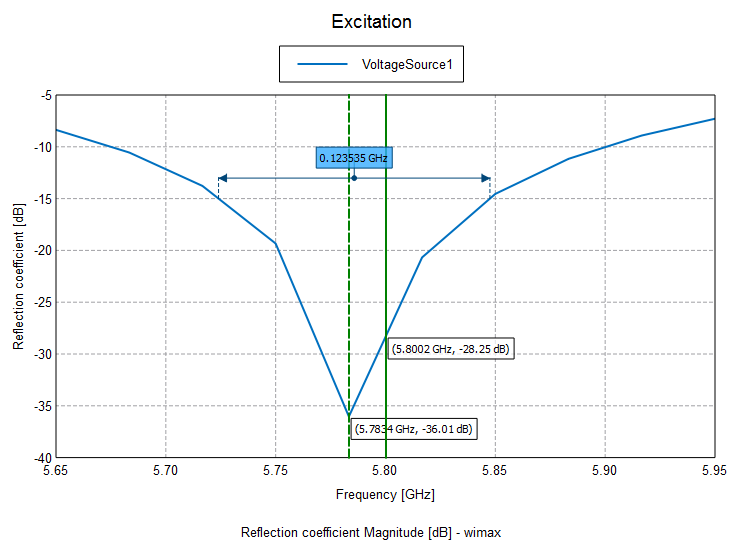
\includegraphics[scale=0.5]{Immagini/reflection_coefficient_optimized}
\end{figure}

Nella figura \ref{img:impopt} sono rappresentati i valori della parte reale e della parte immaginaria dell'impedenza di ingresso, un confronto con i valori precedenti mostra come la parte reale sia di poco inferiore alla precedente $46.1 \Omega$ ma la parte immaginaria sia prossima allo zero $-0.726 \Omega$; molto importante è quest'ultimo valore, dimostra come siano quasi nulle le perdite di potenza dovute all'impedenza d'ingresso. \\[1cm]

\begin{figure}
\centering
\caption{Parte reale e parte immaginaria dell'impedenza adattate alle specifiche di progetto.}
\label{img:impopt}
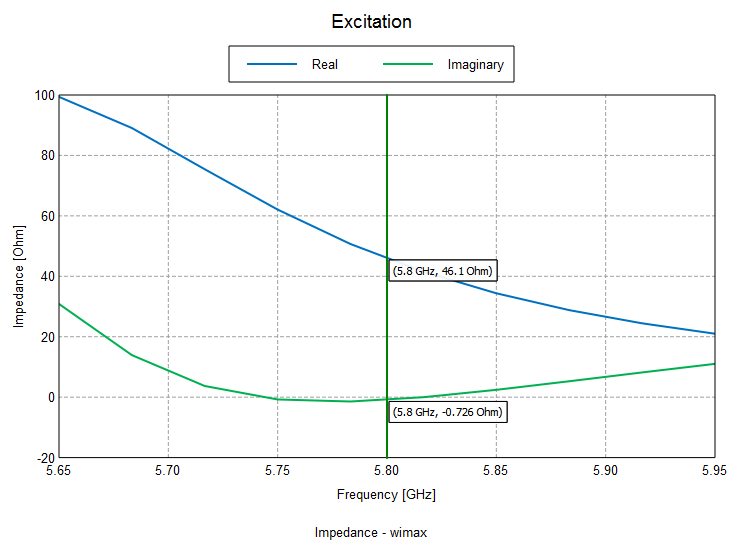
\includegraphics[scale=0.5]{Immagini/impedance_optimized}
\end{figure}

La figura \ref{img:polar}, infine, mostra il diagramma polare del guadagno in dB, sul taglio $E(\phi=\frac{\pi}{2})$ nella direzione di \emph{broadside}, $\theta = \frac{\pi}{2}$. Il guadagno è pari a $7.26 dB$.

\begin{figure}
\centering
\caption{Diagramma polare del guadagno in scala logaritmica.}
\label{img:polar}
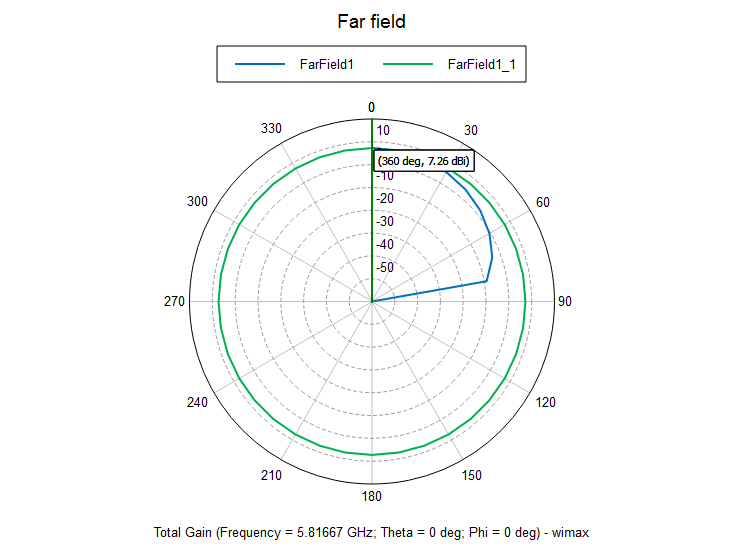
\includegraphics[scale=0.5]{Immagini/total_gain_optimized}
\end{figure}
\section{Progettazione dell'array di patch}
Una volta soddisfatte le specifiche per il singolo patch rettangolare, è necessario cercare di soddisfare anche le restanti, relative all'array. \\ 
Per fare questo è possibile agire su due fattori relativi all'array: il numero degli elementi che formano l'array e la spaziatura tra gli elementi. Per calcolare il numero di elementi che formano l'array ci si deve riferire alla specifica del guadagno massimo dell'array, la relazione che lo lega con il guadagno del singolo patch permette di ottenere il numero di elementi che formano l'array considerando un'illuminazione uniforme.
\begin{align*}
G^{(array)}_{max} = (K+1) G^{(patch)}_{max}
\end{align*}
\begin{align}
\label{eq:m}
\Rightarrow M = K + 1 =  \biggr\lceil \frac{G^{(array)}_{max}}{G^{(patch)}_{max}} \biggr\rceil = \lceil 7.71 \rceil = 8
\end{align}
dove:
\begin{itemize}
\item $G^{(array)}_{max}$ è dato dalla specifica di progetto: $16 dB$
\item $G^{(patch)}_{max}$ è quello ottenuto nella figura \ref{img:polar}: $7.26 dB$
\end{itemize}
Il numero di elementi trovato nell'equazione \ref{eq:m} rappresenta il numero \emph{minimo} di elementi che possono formare l'array a illuminazione uniforme; in questo lavoro, però, si studia la progettazione di un array a illuminazione simmetrica, pertanto la scelta del numero \emph{minimo} di elementi si opera attraverso le seguenti equazioni:
\begin{align}
\label{eq:mopt}
N = \biggr\lceil \frac{M-1}{2} \biggr\rceil = 4 \Rightarrow M = 2N + 1 = 9
\end{align}

Il numero di elementi \emph{minimo} trovato nella (\ref{eq:mopt}) soddisfa il requisito sul guadagno massimo dell'array, quest'ultimo passaggio è stato necessario al fine di poter applicare la sintesi di \cheby. In questo modo sarà possibile calcolare il numero ottimo di elementi che formano l'array e la loro distanza. \\
Restano quindi da soddisfare gli ultimi due requisiti che riguardano \emph{il rapporto tra l'ampiezza massima del lobo principale e quella del lobo secondario} e \emph{l'angolo a metà potenza (BW)}. \\

\subsection{Sintesi di \cheby}
La sintesi di \cheby è stata automatizzata attraverso un programma in Python, di cui è allegato il codice. \\[1cm]

Il primo script contiene le funzioni che calcolano i parametri di \cheby, i coefficienti di alimentazione e il fattore d'array e eseguono la sintesi dando in output tutti i risultati.
\begin{minted}[linenos=true,frame=leftline,xleftmargin=0.5cm,fontsize=\footnotesize]{python}
import math
from pylab import*

# the function takes in input the number of array elements "n" and 
# the attenuation of the secondary lobes compared to the main lobe
def chebyParam( n , r ):
    n = float(n)
    r = float(r)
    iterator = math.cosh(1/n * math.acosh(r))
    a = (( iterator - 1 ) / 2 ).real
    b = (( iterator + 1 ) / 2 ).real
    #returns the list of chebyshev's parameters
    return [ a , b ]

#chebyshev's parameters and optimized distance value btw array elements
def chebyParamOptimized(n , r , k0 ):
    n = float(n)
    r = float(r)
    iterator = math.cosh(1/n * math.acosh(r))
    a = (( iterator - 1 ) / 2 ).real
    b = (( iterator + 1 ) / 2 ).real
    optimized_dist = ( 2*math.pi - math.acos((1 - a)/b)) / k0
    output = open("valori_a_b.txt",'a')
    output.write(" a = " + str(a) + " b = " + str(b) + "  N = " + str( n*2+1) + "\n")
    output.close()
    return [ a , b , optimized_dist]

# the function takes in input the chebyshev's parameters and returns the 
# excitation coefficients

def excitCoeff( n , a, b):
    if n not in range(2,5):
        raise Exception("The number isn't in the range [ 2 , 4 ]")
    # 5 elements array
    def five_elem():
        k0 = 2*a**2 + b**2 - 1
        k1 = 4*a*b/2
        k2 = b**2/2
        return [ k0 , k1 , k2 ]
    #7 elements array
    def seven_elem():
        k0 = 4*a**3 + 6*a*b**2 - 3*a
        k1 = ( 12*a**2*b +3*b**3 - 3*b )/2
        k2 = ( 6*a*b**2 )/2
        k3 = b**3/2
        return [ k0 , k1 , k2 , k3 ]
    #9 elements array
    def nine_elem():
        k0 = -8*a**2 + 8*a**4 - 4*b**2 + 3*b**4 + 24*a**2*b**2 +1
        k1 = (24*a*b**3 + 32*a**3*b - 16*a*b)/2
        k2 = (4*b**4 - 4*b**2 + 24*a**2*b**2)/2
        k3 = 8*a*b**3/2
        k4 = b**4/2
        return [ k0 , k1 , k2 , k3 , k4 ]

    feed_coeff = { 2 : five_elem , 3 : seven_elem , 4 : nine_elem }
    return feed_coeff[n]()

#the function takes in input the excitation coefficients, the distance between array elements, 
#the angle of orientation
#returns the array factor

def arrayFactor( coeff , dist , angle , k0 ):
    u = k0 * dist * cos((angle*pi)/180)
    f = zeros(len(angle))
    for item in range(0,len(angle)):
        f[item] = coeff[0]
        for item2 in range(1,len(coeff)):
            f[item] = f[item] + 2*coeff[item2]*cos(item2*u[item])
    return f


# Chebyshev sysnthesis

def chebyshevSynthesis( f0 , r , angle , gain , n ):

    gain = 10**(array(gain)/10)
    c = float(3*(10**8))
    #wave length
    r = 10**(r/20)
    lambda_0 = c/float(f0)
    k0 = 2*math.pi/lambda_0
    psi = 90 - np.array(angle)
    m = int(ceil(( n-1 )/2))
    params = chebyParamOptimized( m , r , k0)
    excitation_coeff = excitCoeff( m, params[0] , params[1] )
    array_factor = np.array(arrayFactor( excitation_coeff, params[2] , psi , k0))
    #square absolute value of the array factor
    abs_array_factor = abs(np.array(array_factor))**2

    # the sum of the absolute values of the excitation parameters
    sum_coeff = sum( abs(array(excitation_coeff))**2)*2 - abs(excitation_coeff[1])**2 
    
    array_factor_gain = abs_array_factor/float(sum_coeff)
    #the gain of the antenna
    system_gain = array_factor_gain * gain
    db_system_gain = 10*log10(system_gain)

    
    max_gain = max(db_system_gain)
    
    db_3_gain = 0
    teta_3_db = -1

    for  item in range(1, len(angle)):
        if db_system_gain[item] == db_3_gain :
            teta_3_db = angle[item]
            break
        elif db_system_gain[item] < db_3_gain:
            teta_3_db = angle[item - 1]
            break
    

    if teta_3_db == -1 :
        print(" Impossible to calculate the beamwidth ")
    print(teta_3_db)
    bw = 2*teta_3_db

    return [ array_factor , array_factor_gain , system_gain , max_gain , bw ]


def chebySynthesisDistance( f0 , r , angle , gain , n , dist ):
    c = float(3*10**8)
    r = 10**(r/20)
    lambda_0 = c/float(f0)
    k0 = 2*math.pi/lambda_0
    psi = 90 - array(angle)
    m = int(ceil((n-1)/2))
    params = chebyParam( m , r )
    excitation_coeff = excitCoeff( m , params[0] , params[1] )
    array_factor = arrayFactor(excitation_coeff , dist , psi , k0 )
    abs_array_factor = abs(array_factor)**2
    sum_coeff = sum(abs(array(excitation_coeff))**2)*2 - abs(excitation_coeff[1])**2
    array_factor_gain = abs_array_factor/float(sum_coeff)
    system_gain = array_factor_gain*gain
    db_system_gain = 10*log10(system_gain)
    max_gain = max(system_gain)
    db_max_gain = max(db_system_gain)
    db_3_gain = db_max_gain - 3
    print(db_system_gain)
    teta_3_db = -1
    for  item in range(0, len(angle)):
        if db_system_gain[item] == db_3_gain: 
            teta_3_db = angle[item]
            break
        elif db_system_gain[item] < db_3_gain:
            teta_3_db = angle[item - 1]                                                         
            break
        
    if teta_3_db == -1 :
        print(" Impossible to calculate the beamwidth ")

    bw = 2*teta_3_db
    return [ array_factor , array_factor_gain , system_gain , max_gain , bw ]

def plot_function(axes,values , names ):
    m = values[0]
    g=[]
    for item in axes:
        g.append(-1*item)
    g = g[::-1]
    axes = g + axes
    values = array(list(values[::-1])+list(values))
    plot(axes,values)
    ylim(-60,35)
    xlim(-90,90)
    annotate(str(m)[0:5], xy=(5, m+6), xytext=(5, m+6),bbox=dict(boxstyle="larrow", fc="w"), rotation = 35)
    grid(True)

    ylabel(names[0])
    xlabel(names[1])
    title(names[2])
\end{minted}

Il seguente script genera i grafici del fattore d'array e del guadagno totale dell'antenna.
\begin{minted}[linenos=true,frame=leftline,xleftmargin=0.5cm,fontsize=\footnotesize]{python}
import antenna_package
import math
from pylab import*

r = float(20)
f0 = 5.8*10**9
file_gain = open("gainTotal.txt",'r')
file_angles = open("gain_angoli.txt",'r')

gain = []
angles = []
while True:
    line = file_gain.readline()
    if not line:
        break
    gain.append(float(line))
file_gain.close()

while True:
    line = file_angles.readline()
    if not line:
        break
    angles.append(float(line))
file_angles.close()

for item in gain:
    item = 10**item/10

n = [ 5,7,9 ]
array_factors = zeros((len(n),len(gain)))
array_factors_gain = zeros((len(n),len(gain)))
system_gain = zeros((len(n),len(gain)))
max_gain = zeros(len(n))
beam_width = zeros(len(n))
output = open("beamwidth.txt",'wa')
for item in range(0,len(n)):
    synthesis_result = antenna_package.chebyshevSynthesis( f0, r , angles , gain, n[item] )
    array_factors[item] = synthesis_result[0]
    array_factors_gain[item] = synthesis_result[1]
    system_gain[item] = synthesis_result[2]
    max_gain[item] = synthesis_result[3]
    beam_width[item] = synthesis_result[4]

for item in range(0,len(n)):
    output.write("N = " + str(n[item]) + " bw = " + str(beam_width[item]) + "\n")
output.close()
max_gain_db = 10*log10(max_gain)
array_factors_abs = abs(array_factors)
array_factors_abs_db = 20*log10(array_factors_abs)
array_factors_gain_db = 10*log10(array_factors_gain)
system_gain_db = 10*log10(system_gain)

g = []
for item in angles:
    g.append(-1*item)
g=g[::-1]
axes = g + angles
a = list(array_factors_abs_db[2][::-1]) + list(array_factors_abs_db[2])

for item in range(0,len(n)):
    names_array_factors = [ "db","angle","Array factor absolute value for " + str(n[item]) + " elements"]    
    figure()
    antenna_package.plot_function(angles,array_factors_abs_db[item],names_array_factors)
    show()
    names_system_gain = ["db","angle"," Gain of the " + str(n[item]) + " elements array patch antenna"]
    figure()
    antenna_package.plot_function(angles,system_gain_db[item],names_system_gain)
    show()
\end{minted}

L'ultimo script genera i grafico dell'andamento del beamwidth in funzione della spaziatura tra i patch.
\begin{minted}[linenos=true,frame=leftline,xleftmargin=0.5cm,fontsize=\footnotesize]{python}
import antenna_package
import math
from pylab import*

n = 5
c = 3.0*10**8
r = 20.0
f0 = 5.8*10**9
lambda_0 = c/f0

file_gain = open("gainTotal.txt",'r')
file_angles = open("gain_angoli.txt",'r')

gain = []
angles = []
while True:
    line = file_gain.readline()
    if not line:
        break
    gain.append(float(line))
file_gain.close()

while True:
    line = file_angles.readline()
    if not line:
        break
    angles.append(float(line))
file_angles.close()

for item in range(0,len(gain)):
    gain[item] = 10**(gain[item]/10)

#distances between array elements
distances = arange(lambda_0/2,lambda_0,0.01)
array_factor = zeros((len(distances),len(angles)))
array_factor_gain = zeros((len(distances),len(angles)))
system_gain = zeros((len(distances),len(angles)))
max_gain = zeros(len(distances))
beam_width = zeros(len(distances))

for item in range(0,len(distances)):
    synthesis_results =  antenna_package.chebySynthesisDistance(f0, r , angles, gain, n, distances[item])
    synthesis_results[0]
    array_factor[item] = synthesis_results[0]
    array_factor_gain[item] = synthesis_results[1]
    system_gain[item] = synthesis_results[2]
    max_gain[item] = synthesis_results[3]
    beam_width[item] = synthesis_results[4]
print(len(beam_width))
print(len(distances))
plot(distances,beam_width)
grid(True)
xlabel( "distance between pathces" )
ylabel(" beamwidth")
title(" Beamwidth variation for " + str(n) + " elements array antenna " )
show()
\end{minted}

\subsection{Risultati}
I risultati della sintesi di \cheby sono contenuti in grafici che rappresentano il guadagno del fattore di array, il guadagno totale del patch e dell'array e l'angolo a metà potenza. Per ognuna di queste tre tipologie è stato considerato un numero di elementi dell'array variabile: $M = 5, 7, 9 $. \\
Si è inoltre considerata la spaziatura ottima tra gli elementi, utilizzando i valori ottenuti dalla sintesi di \cheby (Tab. \ref{tab:ab}) mediante la formula:
\begin{align}
\label{eq:d}
d_{ottima} = \frac{2 \pi - arcos(\frac{1-a}{b})}{k_0}
\end{align}

\begin{table}[h]\footnotesize
\caption{Valori di $a$ e $b$ ottenuti dalla sintesi di \cheby.}
\label{tab:ab}
\begin{tabularx}{\textwidth}{XXXXXX}
\toprule
& $M = 5$ & $M = 7$ & $M = 9$ \\
\midrule
a & 0.672603939956 & 0.270214865098 & 0.146645950261 \\
b & 1.67260393996 & 1.2702148651 & 1.14664595026 \\
\bottomrule
\end{tabularx}
\end{table}

Nei grafici che rappresentano il modulo del fattore di array (Fig. \ref{img:module5}, \ref{img:module7}, \ref{img:module9}) e il guadagno totale (Fig. \ref{img:gain5}, \ref{img:gain7}, \ref{img:gain9}) si è considerata una spaziatura $d$ fissa, calcolata per $M = 5, 7, 9$. \\[1cm]
Nelle figure \ref{img:module5}, \ref{img:module7}, \ref{img:module9} è mostrato il modulo del fattore di array per $M = 5, 7, 9$. Si può vedere chiaramente come all'aumentare di M aumentino il numero di lobi secondari, ma altrettanto evidente è la differenza, \emph{in dB}, tra il lobo principale e il lobo secondario. \\
In ogni grafico, quindi per ogni $M$, si può vedere come sia soddisfatta la specifica su R, la quale era richiesta essere di $-20dB$, tale, infatti, è la differenza in ampiezza tra il lobo principale e quelli secondari, che sono invece fermi a $0dB$. \\[1cm]

\begin{figure}
\centering
\caption{Modulo del fattore di array per M = 5.}
\label{img:module5}
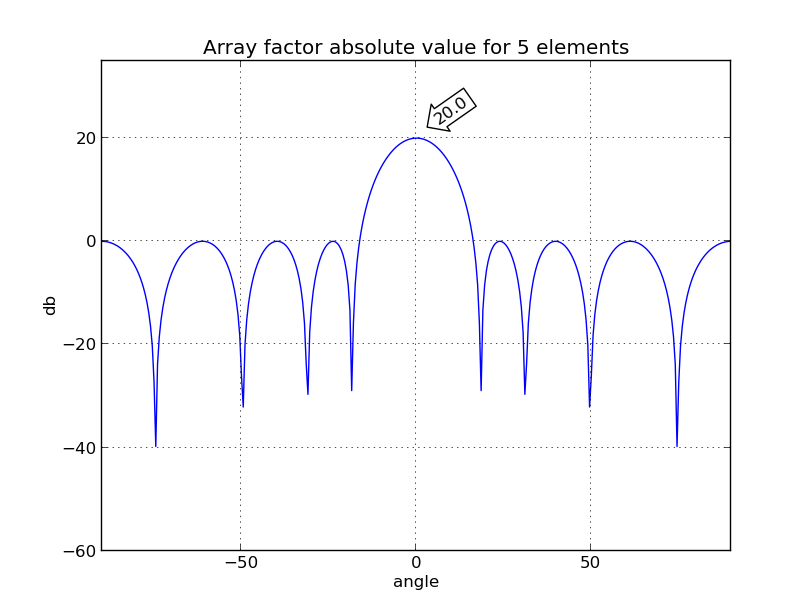
\includegraphics[scale=0.5]{Immagini/module5}
\end{figure}
\begin{figure}
\centering
\caption{Modulo del fattore di array per M = 7.}
\label{img:module7}
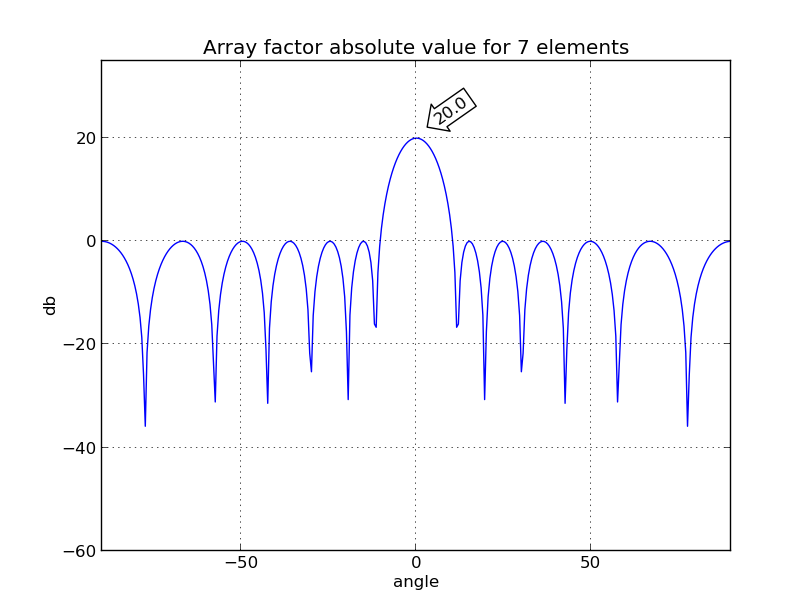
\includegraphics[scale=0.5]{Immagini/module7}
\end{figure}
\begin{figure}
\centering
\caption{Modulo del fattore di array per M = 9.}
\label{img:module9}
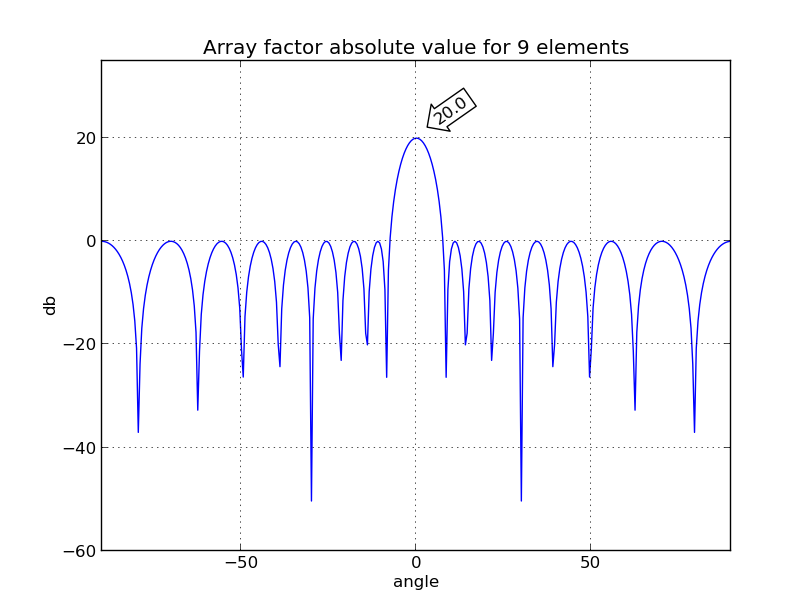
\includegraphics[scale=0.5]{Immagini/module9}
\end{figure}

Per quanto riguarda il guadagno totale del patch e dell'array (Fig. \ref{img:gain5}, \ref{img:gain7}, \ref{img:gain9}), si può vedere come all'aumentare di $M$ diminuisca la larghezza dei lobi (in particolare di quello principale) e aumenti il numero di lobi secondari. Molto importante è anche l'aumento del guadagno che arriva ad un valore prossimo a $16 dB$ (come previsto dalle specifiche) per $M = 9$, avendolo impostato nella relazione (\ref{eq:m}). \\ 

\begin{figure}
\centering
\caption{Guadagno totale per M = 5.}
\label{img:gain5}
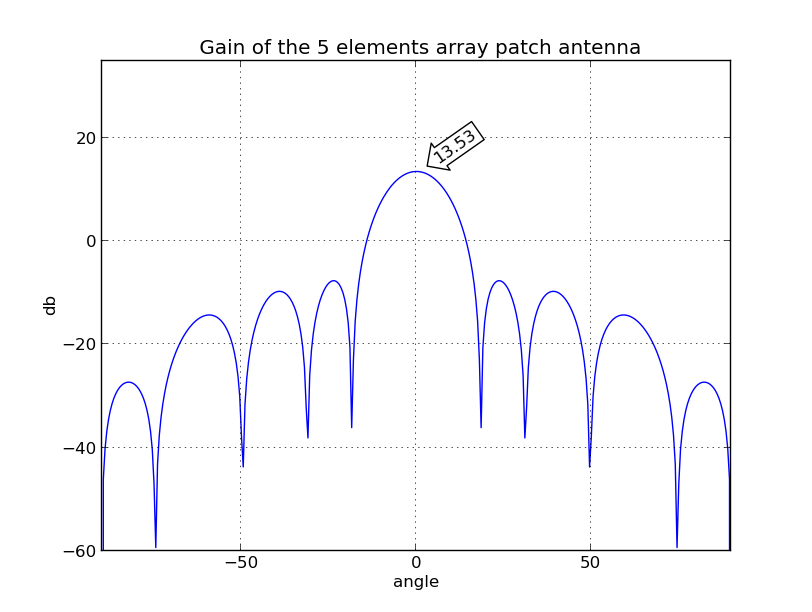
\includegraphics[scale=0.5]{Immagini/gain5}
\end{figure}
\begin{figure}
\centering
\caption{Guadagno totale per M = 7.}
\label{img:gain7}
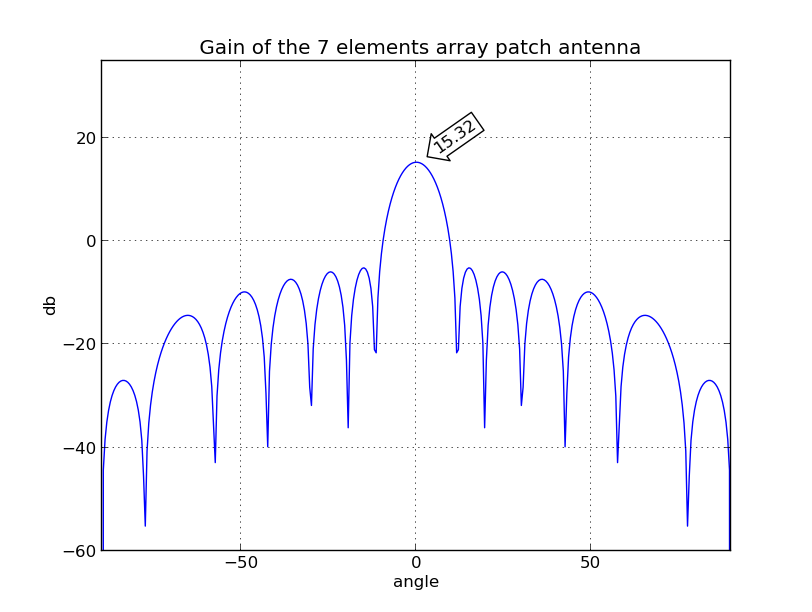
\includegraphics[scale=0.5]{Immagini/gain7}
\end{figure}
\begin{figure}
\centering
\caption{Guadagno totale per M = 9.}
\label{img:gain9}
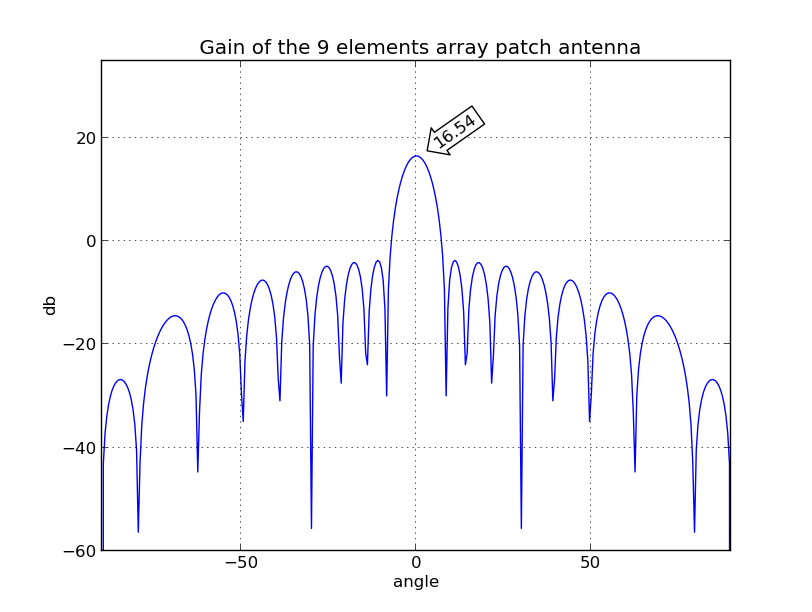
\includegraphics[scale=0.5]{Immagini/gain9}
\end{figure}


Infine è stata fatta variare la distanza tra gli elementi dell'array (tra $\frac{\lambda}{2}$ e $\lambda$) ed è stato rappresentato il beamwidth; in ognuno dei tre grafici è stata considerata una diversa cardinalità degli elementi degli array, $M = 5$ (Fig. \ref{img:bw5}), $7$ (Fig. \ref{img:bw7}), $9$ (Fig. \ref{img:bw9}). \\
Si può notare chiaramente come il \emph{beamwidth} diminuisca all'aumentare della distanza tra gli elementi. Per capire se sia soddisfatta la specifica sull'angolo a metà potenza è necessario controllare il valore di $10^\circ$ del \emph{beamwidth}: nel caso di $M = 5$ nel range considerato di $d$ non è possibile trovare il \emph{beamwidth} richiesto, al contrario che nelle altre due configurazioni. In particolare si può notare come nel caso di $M = 9$ la scelta di $d$ sia diversa da quella calcolata con la (\ref{eq:d}) ma nonostante questo, si può scegliere il relativo valore a $B = 10^\circ$, in quanto le specifiche su $R$ e su $G$, restano soddisfatte perché indipendenti dalla distanza $d$. \\[1cm]
\begin{figure}
\centering
\caption{Angolo a metà potenza per M = 5.}
\label{img:bw5}
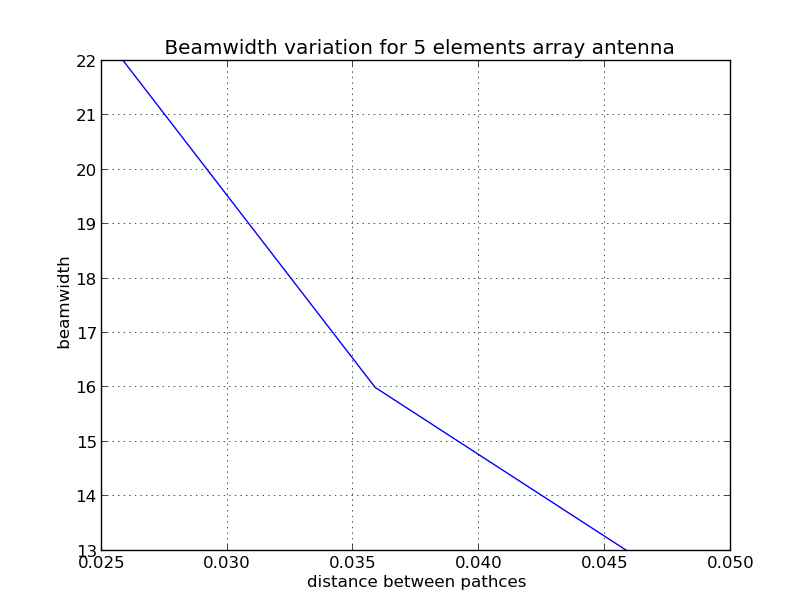
\includegraphics[scale=0.5]{Immagini/bw5}
\end{figure}
\begin{figure}
\centering
\caption{Angolo a metà potenza per M = 7.}
\label{img:bw7}
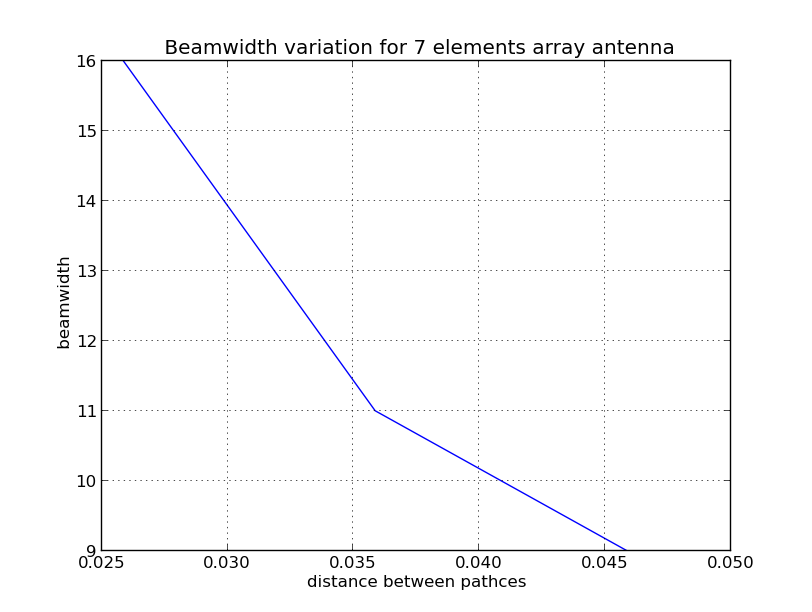
\includegraphics[scale=0.5]{Immagini/bw7}
\end{figure}
\begin{figure}
\centering
\caption{Angolo a metà potenza per M = 9.}
\label{img:bw9}
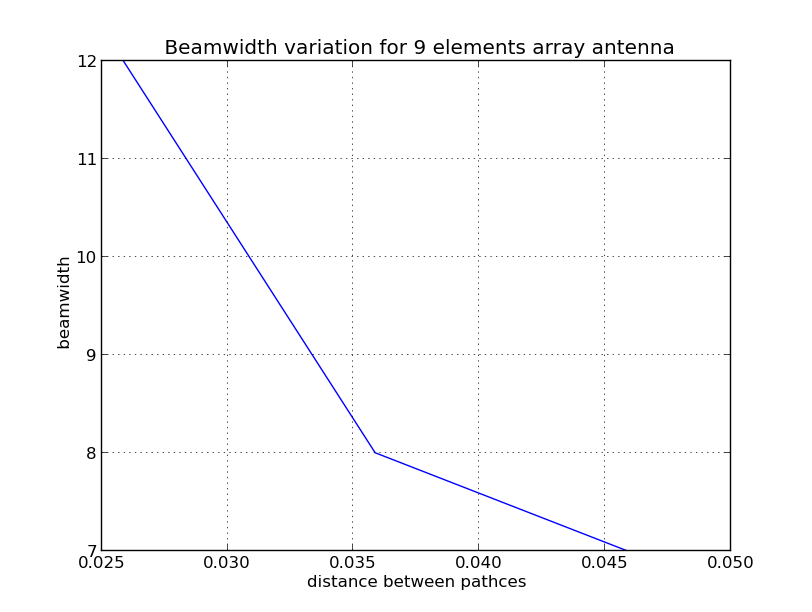
\includegraphics[scale=0.5]{Immagini/bw9}
\end{figure}

Nella tabella \ref{tab:dgbopt} sono riassunti i risultati ottenuti nelle tre tipologie di grafico rappresentate nelle pagine precedenti, in funzione della cardinalità degli elementi dell'array.
\begin{table}[h]\footnotesize
\caption{Risultati al variare di M.}
\label{tab:dgbopt}
\begin{tabularx}{\textwidth}{XXXX}
\toprule
& $M = 5$ & $M = 7$ & $M = 9$ \\
\midrule
Distanza ottima (m) & 0.0404149389796 & 0.043831493932 & 0.0457028645254 \\
Guadagno max	 (dB) & 13.53 & 15.32 & 16.54 \\
Beamwidth & $14.0^\circ$ & $9.0^\circ$ & $7.0^\circ$ \\
\bottomrule
\end{tabularx}
\end{table}

\newpage
% *****************************************************************
% Materiale finale
%******************************************************************
\section{Conclusioni}
Lo studio effettuato nelle pagine precedenti mostra come la scelta ideale sia quella di $M = 9$ e $d = 0.031 m$, questa scelta deriva dai risultati mostrati nei grafici \ref{img:module9}, \ref{img:gain9}, \ref{img:bw9}. \\
Il primo mostra infatti come la specifica sulla differenza in $dB$ tra il lobo principale e quello secondario, $R$, sia soddisfatta. \\
La seconda evidenzia il guadagno massimo del patch e dell'array, $16.54 dB$, come da specifica; mentre nel terzo si vede chiaramente come la scelta di $0.031 m$ per la distanza tra gli elementi dell'array sia ideale per ottenere un angolo a metà potenza pari a $10^\circ$. \\[1cm]
Un'ulteriore scelta potrebbe essere $M = 7$ con la distanza ottima calcolata nella (\ref{eq:d}), $d = 0.043831493932$, questa scelta soddisferebbe sicuramente i requisiti su $R$ e $B$, ma il guadagno sarebbe di circa $0.7 dB$ inferiore a quello richiesto.
\end{document}
